\chapter{Network Flow Monitoring}

\itodo{Fix all references}

The article of \citeauthor{Hofstede-2014-Flow}~\cite{Hofstede-2014-Flow} extensively covers the topic of flow monitoring process and much information provided in this chapter is influenced by it. The reader is encouraged to study the article, the relevant sections are II to VIII with the exception of section VII. However, this chapter explains the flow monitoring process in the context of this thesis, therefore some aspects of the flow monitoring, such as flow export processes, are described in more detail.

\section{Flow Monitoring Basics}

This section describes history and current state of network flow monitoring. We discuss related standards, introduce terminology used throughout this thesis and provide formal definition of a flow. 

\subsection{History of Flow Monitoring}

The first mention of flow export can be found in RFC 1272~\cite{rfc1272} published in 1991 by IETF Internet Accounting (IA) Working Group (WG). The goal of the document was to provide background information on Internet accounting. The authors describe methods of metering and reporting network utilization. The RFC defines a metering process as follows:

\begin{displaycquote}{rfc1272}[Internet accounting: Background]
A METER is a process which examines a stream of packets on a communications medium or between a pair of media. The meter records  aggregate counts of packets belonging to FLOWs between communicating entities (hosts/processes or aggregations of communicating hosts (domains)).
\end{displaycquote}

The goal at the time was to provide a framework for traffic accounting, however, the common believe at the time was that internet should be free and any form of traffic capture, even for the accounting purposes, is undesirable. This, together with the lack of vendor interest, resulted in the conclusion of the working group in 1993. Note that the negative attitude towards the monitoring returns more than 20 years later~\cite{rfc7258}.

In 1995, \citeauthor{Claffy-1995-Parameterizable} showed a methodology for internet traffic flow profiling based on packet aggregation~\cite{Claffy-1995-Parameterizable}, which started a revival of flow monitoring efforts. The Realtime Traffic Flow  Measurement (RTFM) Working Group was created in 1996 and it had three main objectives. First was to consider current issues relating to traffic measurement, such as security, privacy, policies and requirements on new network protocols. Second was to produce an improved Traffic Flow Model that should provide a wider range of measurable quantities (e.g. IPv6), simpler way to specify flows of interest, better access control  to measured flow data, strong focus on data reduction capabilities and efficient hardware implementation. The third objective was to develop RTFM Architecture and Meter Management Information Base (MIB) as a standards track IETF documents. The effort resulted in 1999 by publishing several RFCs describing new traffic flow measurement framework with an increased flexibility and even a bi-directional flow support~\cite{rfc2722}. Since these documents fulfilled the objectives of the RTFM WG, the group was concluded in 2000. However, no flow export standard was developed as the vendors showed no interest in this area.

Meanwhile, Cisco realized that similar kind of flow information is already stored in a flow cache of their packet switching devices. The purpose of this cache is to speed up packet switching by making a forwarding decision only for the first packet of each flow. Unlike the RTFM flow measurement framework, the primary purpose of flow cache is not accounting nor monitoring, therefore the configuration of measurement process using a flow cache in a switch is severely limited. Despite the limitations, once Cisco introduced its own flow export technology called NetFlow, it achieved widespread adoption. The main reason for the extensive adoption was the fact that it was readily available in most Cisco devices with little effort. The NetFlow was patented in 1996 and the first version that became available to general public around 2002 was NetFlow v5~\cite{CiscoSystems-2007-NetFlow}, albeit Cisco newer released any official specification. The NetFlow v5 format simply specified a single set of fields that should be exported from each flow record. Figure~\ref{fig:nf5-fields} shows all fields that were supported by NetFlow v5. Note the lack of support for IPv6 protocol.

\begin{figure}[t!]
  \begin{center}
    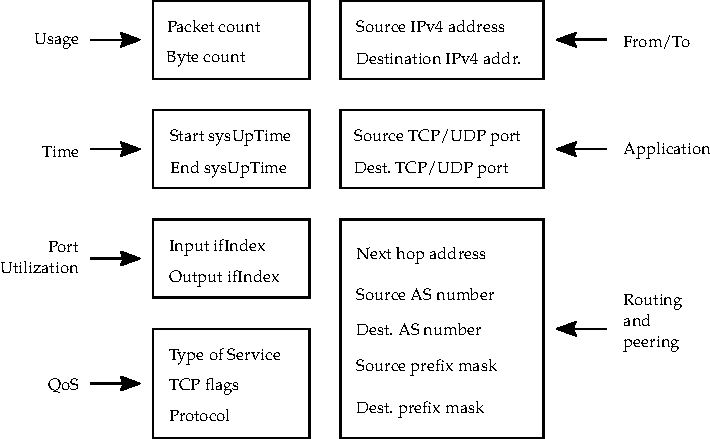
\includegraphics[width=\textwidth]{figures/nf5-fields}
  \end{center}
  \caption{NetFlow v5 Fields}
  \label{fig:nf5-fields}
\iimprove{add citation}
\iimprove{redraw}
% [nfv5-fields] http://www.cisco.com/c/en/us/td/docs/ios/solutions_docs/netflow/nfwhite.html
% http://www.cisco.com/c/dam/en/us/td/i/000001-100000/60001-65000/60001-61000/60682.ps/_jcr_content/renditions/60682.jpg
\end{figure}

The NetFlow version 5 was soon obsoleted by NetFlow version 9 which remedied some of the deficiencies of the previous version. The state of NetFlow v9 is described in~\cite{rfc3954}. It allowed to define arbitrary set of fields for export using templates as shown in Figure~\ref{fig:nf9-protocol}. It also introduced support for new protocols, such as IPv6, Virtual Local Area Networks (VLAN), Multiprotocol Label Switching (MPLS), Border Gateway Protocol (BGP) or Multicast. 

\begin{figure}[t!]
  \begin{center}
    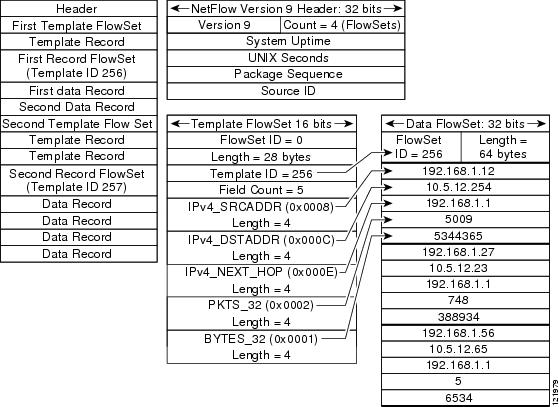
\includegraphics[width=\textwidth]{figures/nf9-protocol}
  \end{center}
  \caption{NetFlow v9 Structure Example}
  \label{fig:nf9-protocol}
\iimprove{add citation}
\iimprove{redraw}
% [nfv9-format] http://www.cisco.com/c/en/us/td/docs/ios/solutions_docs/netflow/nfwhite.html
% http://www.cisco.com/c/dam/en/us/td/i/100001-200000/120001-130000/121001-122000/121979.ps/_jcr_content/renditions/121979.jpg
\end{figure}

Other vendors created their own versions of flow exporting protocols, although they retained some level of compatibility with NetFlow. There are JFlow by Juniper, CFlow by Alcatel-Lucent, RFlow by Ericsson, and other protocols. When the potential of flow monitoring for security purposes became realized~\cite{CiscoSystems-2005-Cisco} in 2005, more effort was devoted to extend flow records with information not directly associated with switching. Cisco presented Flexible NetFlow technology~\cite{CiscoSystems-2008-Cisco} in 2006 which allows to dynamically define and export new types of information, such as parts of payloads or traffic identification.

In 2001, it was clear that exporting flow information from switching devices is going to be supported by vendors. However, no standard flow export protocol existed at the time and NetFlow v5 was not yet released to general public. For that reason the IETF started IP Flow Information Export (IPFIX) WG~\cite{IETF--IP}. The original charter~\cite{IESG-2001-IP} defined six specific goals for the WG: 

\begin{itemize}
	\item Define \emph{``standard IP flow''}.
	\item Devise flow data encoding that support multiple levels of aggregation.
	\item Allow packet sampling in IP flow.
	\item Identify and address security and privacy concerns affecting flow data.
	\item Specify the transport mapping for IP flow information.
	\item Ensure that the flow export system is reliable.
\end{itemize}

The charter was updated over the years to match current requirements. Several vendors were engaged in the IPFIX WG’s activities, most notably Cisco, which significantly contributed from the start. The WG defined set of requirements for the IPFIX protocol~\cite{rfc3917} and evaluated existing candidate protocols~\cite{rfc3955} to decide the most suitable approach in defining the new protocol. The NetFlow v9 specification (RFC 3954) was designed with IPFIX requirements in mind~\cite{Trammell-2011-Introduction} and was released in order to compete in this evaluation (RFC 3955). After the evaluation the NetFlow v9 was chosen as a basis of the new IPFIX protocol. For this reason, the IPFIX is sometimes called NetFlow v10 and even starts with protocol version 10 in its header. However, the IPFIX protocol supports many new features and is not completely backwards compatible with NetFlow.

The IPFIX WG did more than just design the IPFIX protocol. In the 29 RFCs submitted before its conclusion, the WG paid attention to e.g.:
\begin{itemize}
	\item Bidirectional flow export~\cite{rfc5103}
	\item Architecture for IP flow information export~\cite{rfc5470}
	\item Reducing redundancy in flow~\cite{rfc5473}
	\item Definitions of Managed Objects (MIB) for IPFIX~cite{rfc5815, rfc6615}
	\item IP flow mediation framework~\cite{rfc5982, rfc6183}
	\item IP flow anonymization~\cite{rfc6235}
	\item IPFIX configuration data model~\cite{rfc6728}
\end{itemize}
The IPFIX protocol specification is described by \emph{``Specification of the IP Flow Information Export (IPFIX) Protocol for the Exchange of Flow Information''}~\cite{rfc7011} which became an Internet Standard. The working group was concluded in 2014, however, IPFIX related Internet-Drafts are still being created by involved parties. Further information about IPFIX development is provided by \citeauthor{Brownlee-2011-Flow} in \cite{Brownlee-2011-Flow}.

\subsection{Related Technologies}

Flow monitoring is not the only network monitoring system used to gain information about network behavior. There are other technologies that can be used to monitor network traffic and that can be sometimes confused with flow monitoring. We describe sFlow~\cite{Phaal-2004-sFlow}, IETF Packet Sampling, OpenFlow and Deep Packet Inspection in the following text.

sFlow is an industry standard that is supported by number of vendors in their packet switching devices. Its initial specification was published as an Informational RFC~\cite{rfc3176} in 2001, which was the time when packet switching/routing devices with sFlow support became available. The most crucial difference from flow monitoring is that the sFlow does not actually aggregate a stream of packet into a flow record. Instead, it uses sampling to select individual packets and then exports information available about and from these packets. sFlow allows to export data from packet headers, chunks of data from packets and even parse application payloads. It also maintains interface counters and allows their regular export, which is a feature completely unrelated to flow monitoring. sFlow version 5 is the latest version and was published in ~\citeyear{Phaal-2004-sFlow}~\cite{Phaal-2004-sFlow}.

In 2002 the IETF started Packet Sampling (PSAMP) Working Group~\cite{IETF--Packet} which was chartered to define a standard set of capabilities for network elements to sample subsets of packets by statistical and other methods~\cite{IESG--Packet}. The result is similar to sFlow, however, the PSAMP uses IPFIX protocol for data export~\cite{rfc5477}. The WG was concluded in 2009 after publishing four RFCs. The proposed standards include sampling and filtering techniques for IP packet selection~\cite{rfc5475}, packet sampling protocol specifications~\cite{rfc5476} and information model for packet sampling export~\cite{rfc5477}.

OpenFlow~\cite{ONF-2012-OpenFlow} is an open-source implementation of the Software Defined Networking (SDN) concept~\cite{Singh-2017-Survey, Hu-2014-Survey}. The idea of SDN is to separate control plane and data plane of networking devices. This means that the packet forwarding rules are known only to SDN controllers. The other networking devices that process the traffic ask the controllers what to do with individual flows. After the decision is made for the first packet of the flow, a flow record is kept in the cache so that subsequent lookups do not require the controller interaction. The OpenFlow is a protocol of communication between the networking devices and the controllers. It has been shown by \citeauthor{Yu-2013-FlowSense}~\cite{Yu-2013-FlowSense} that the information stored in the flow caches can be exported using the OpenFlow protocol to the controller and used for network monitoring. Although the approach to network monitoring is somewhat similar to flow monitoring on non-SDM networking devices, there are significant differences. The control traffic itself is utilized to transfer data about new and expired flow records. Therefore, configuration of flow monitoring is directly affected by configuration of SDN network and vice versa. This imposes undesirable restrictions on the flow monitoring process. Moreover, the distributed architecture of the monitoring is tightly coupled with the deployment of the network controllers. For these reasons, this thesis does not consider SDN specific flow monitoring. It should be noted, that the SDN enabled networking devices can still export valid flow data as defined by the IPFIX standard. In such a case, the SDN capabilities are irrelevant for flow monitoring purposes.

Deep Packet Inspection (DPI) is an approach to network data analysis where each packet is dissected up to and including application layer protocol (i.e. packet payload). Although this requires much greater resources than standard flow monitoring, it provides maximum information about network traffic. DPI an approach, rather than specific technology, therefore the means of packet capture and information export depend on the particular deployment. For example, sFlow uses DPI to gain information about application layer from packet payloads and exports this information as part of the sFlow protocol. Despite the DPI being diametrically different to flow monitoring, it is being integrated to flow monitoring process to provide the application visibility. This merge balances the detailed view of DPI to fast and scalable architecture of the flow monitoring. This thesis describes how the DPI is integrated to flow monitoring to create Application Flow Monitoring. Neither sFlow nor OpenFlow are not discussed any further in this work and PSAMP is only mentioned as a packet sampling protocol that can be optionally applied to flow monitoring.


\section{Flow Definition}

To be able to accurately describe the flow monitoring process, we need to have a precise definition of what a flow is. The NetFlow v9 description in~\cite{rfc3954} uses the following definition:

\begin{displaycquote}{rfc3954}[Cisco Systems NetFlow Services Export Version 9]

    An IP Flow, also called a Flow, is defined as a set of IP packets
    passing an Observation Point in the network during a certain time
    interval. All packets that belong to a particular Flow have a set of
    common properties derived from the data contained in the packet and
    from the packet treatment at the Observation Point.

\end{displaycquote}

The Observation Point is defined as a location where IP packets can be observed. The definition says that a flow is a set of packets within certain time span. Furthermore, the packets in a flow have a set of common properties and these properties are either derived from data contained in the packet data or from packet treatment (e.g. next hop IP address or input interface). Although this definition is quite generic, it easily covers all common flow creation techniques.

The IPFIX Protocol is an internet standard~\cite{rfc7011} with its own definition of a flow that builds upon the NetFlow v9 definition. It tries to specify what “properties derived from data contained in packet data” means and differentiates two types of data. The first are the values contained in packet headers, the second type covers the characteristics of the packet itself (e.g. packet length). The definition is as follows:

\begin{displaycquote}{rfc7011}[Specification of the IPFIX Protocol]

    A Flow is defined as a set of IP packets passing an Observation
    Point in the network during a certain time interval.  All packets
    belonging to a particular Flow have a set of common properties.
    Each property is defined as the result of applying a function to
    the values of:

    \begin{enumerate}
    \item one or more packet header fields (e.g., destination IP
        address), transport header fields (e.g., destination port
        number), or application header fields (e.g., RTP header fields
        [5]).

    \item one or more characteristics of the packet itself (e.g., number
        of MPLS labels)

    \item one or more fields derived from packet treatment (e.g., next
        hop IP address, output interface)
	\end{enumerate}
        
    A packet is defined as belonging to a Flow if it completely
    satisfies all the defined properties of the Flow.

\end{displaycquote}

Although this definition is a part of the IPFIX internet standard, there are several problems:
\begin{enumerate}
	\item It is not clear what a \emph{packet header} is. One interpretation is that it includes all protocol headers in the packet up to the packet payload (i.e. application layer). However, the transport header is mentioned explicitly and the example indicates that it can also mean only network layer, in which case the data link layer is completely ignored.
	\item The \emph{characteristics of the packet} are not sufficiently described. One can interpret this as anything that cannot be computed directly from the packet header fields. The example states that a number of certain types of headers is considered as part of packet characteristics. The total packet length can be also included here (it was event used as an example in the early drafts in 2002).
	\item The whole IPFIX standard focuses on IP flows. However, the IPFIX export protocol can be used for other purposes as well, such as exporting MIB variables~\cite{rfc6615} or monitoring of ethernet layer~\cite{Hofstede-2011-Flow}. Therefore the generic flow definition should allow even non-IP packets. Note that the NetFlow v9 definition of flow explicitly defines IP flows.
	\item Flows using transport header fields cannot be correctly defined for fragmented IP packets, since transport layer information is present only in the first packet fragment. The NetFlow v9 definition states that the properties are \emph{derived} from packet data, therefore, it does not rule out a use of a cache for correctly assigning or reassembling fragmented packets to correct flow. However, the use of the word \emph{function} in the IPFIX definition limits what can be done with the values of the header fields.
\end{enumerate}

In order to provide the most complete definition of flow, we must address all the above mentioned issues. The most direct solution is to start with the NetFlow v9 definition, allow non-IP packets and be more clear about deriving data from previous packets of the same flow which is used for correct handling of the packet fragmentation. Therefore, the definition used in this thesis is as follows:

\begin{definition}\label{def:flow}

    A \emph{flow} is defined as a sequence of packets passing an \emph{observation point}
    in the network during a certain time interval. All packets that belong
    to a particular \emph{flow} have a set of common properties derived from
    the data contained in the packet, previous packets of the same \emph{flow},
    and from the packet treatment at the \emph{observation point}.

\end{definition}

There are two more terms connected to flow that need to be defined: \emph{flow keys} and \emph{flow records}. The IPFIX definition of the Flow Key needs to be adapted to our definition of flow. We can conveniently shorten the definition to the following:

\begin{definition}\label{def:flow-key}

    Each of the common properties that is used to specify a~\emph{flow} is called a~\emph{flow key}.

\end{definition}

A flow record is basically a tuple containing flow keys and other properties measured for the flow. The following definition reflects that:

\begin{definition}\label{def:flow-record}

    A~\emph{flow record} is a tuple describing particular \emph{flow} containing values of:

    \begin{enumerate}
    	\item all \emph{flow keys} used to specify the \emph{flow},
    	\item other properties of the \emph{flow} derived from:
    	\begin{enumerate}
    		\item data contained in the packets of the \emph{flow},
    		\item the packet treatment of the \emph{flow} at the \emph{observation point}.
    	\end{enumerate}
    \end{enumerate}

\end{definition}

To make the definitions above more clear, we now give an example of concrete properties that might be contained in a flow record. Table~\ref{tab:flow.properties} shows examples of flow record properties that can be derived from packet data and packet treatment. The properties can be aggregated when the derived value differs between individual packets of the flow or where counters such as number of packets are involved. Summary function is usually applied to number of bytes of of each packet, TCP flags are aggregated using logical OR function, flow start timestamp is derived using minimum function on each packet timestamp. The non-aggregated properties may be used as flow keys.

\begin{table}[ht!]
	\centering
	\begin{tabular}{lll}
	\toprule
	                                           & \textbf{Aggregated properties}  & \textbf{Non-aggregated properties}  \\ \midrule
	\multirow{3}{*}{\textbf{Packet data}}      & Number of bytes                 & Source IP address                   \\ 
	                                           & TCP flags                       & Destination port                    \\ 
	                                           & Time to Live                    & Transport protocol                  \\ \midrule
	\multirow{2}{*}{\textbf{Packet treatment}} & Number of packets               & Input interface number              \\ 
	                                           & Flow start timestamp            & Next-Hop IP address                 \\ \bottomrule
	\end{tabular}
	\caption{Examples of Flow Properties}
	\label{tab:flow.properties}
\end{table}

The Definition~\ref{def:flow} states what the flow is. However, although we tried to be as explicit as possible, the definition is informal and therefore subject to different interpretations. For this reason we now provide a formal definition of flow, which not only refines the informal definition, but also provides a guide to construction of the flows.

\begin{defnn}
Let $P$ be a set of all packets. Let $T$ be a set of packet treatment information. We define a set of extended packets
\begin{equation*}
	\widehat{\mathcal{P}} = P\times T,
\end{equation*}
so that $\widehat{p} \in \widehat{\mathcal{P}}$ denotes a packet $p$ together with its packet treatment information. Let $\mathbb{S}$ be a set of indexes of packets observed at an \emph{observation point}:
\begin{equation*}
	\mathbb{S} = \{1, \ldots, n\} \lor \mathbb{N},
\end{equation*}
where $n \in \mathbb{N}$ is the number of observed packets when the number is finite.

We denote sequence of packets and extended packets observed at an \emph{observation point} respectively:
\begin{align*}
	\mathcal{P} &= (p_i)_{i \in \mathbb{S}},\, p_i \in P,\\
	\widehat{\mathcal{P}} &= (\widehat{p}_i)_{i \in \mathbb{S}},\, \widehat{p}_i \in \widehat{P}.
\end{align*}
\end{defnn}
Both sequences are of size $|\mathbb{S}|$. 

Let us now define a \emph{flow selection function} $\varphi$ which takes a sequence of extended packets and a new extended packet and decides whether they form a flow. We will use this function to determine whether a newly observed packet belongs to an existing flow.
\begin{defn}
Let $\widehat{P}^*$ be a set of all finite sequences of extended packets, $\widehat{P}$ be a set of extended packets. We say that a function of type
\begin{equation*}
 	\varphi: \widehat{P}^*\times \widehat{P} \to \{true,false\}
\end{equation*}
is a \emph{flow selection function}.
\end{defn}

Before we give a formal definition of a flow, we provide the following intuition for our definition. A flow $\mathcal{F}$ is a sequence of packets defined by a sequence of extended packets with indexes in $\mathbb{S}$ and a flow selection function $\varphi$. We require whether each packet belongs to the flows is determined by all previous packets of that flow, therefore we construct the flow by induction as described in Algorithm~\ref{alg:flow-construction}.
% \begin{enumerate}[noitemsep]
% 	\item Denote $\mathbb{I}$ the set of indexes of packets that belong to the flow $\mathcal{F}$\improve{rewrite as an algorithm}
% 	\item Start with $\mathbb{I} = \emptyset$
% 	\item Find the index $k$ of the first extended packet $\widehat{p}_k$ for which the flow selection function $\varphi((\widehat{p}_n)_{n\in J_{i-1}}, \widehat{p}_{\alpha})$ returns true and add $k$ to $\mathbb{I}$
% 	\item Repeat step 3 until no such $k$ exists
% 	\item The flow $\mathcal{F}$ is a sequence of packets with indexes in $\mathbb{I}$
% \end{enumerate}
\begin{algorithm}
    \caption{Construction of flow}
    \label{alg:flow-construction}
    \begin{algorithmic}[1]
        \STATE Denote $\mathbb{I}$ the set of indexes of packets that belong to the flow $\mathcal{F}$
        \STATE Start with $\mathbb{I} = \emptyset$
        \REPEAT 
			\STATE Find the index $k$ of the first extended packet $\widehat{p}_k$ for which the flow selection function $\varphi((\widehat{p}_n)_{n\in J_{i-1}}, \widehat{p}_{\alpha}) = true$
			\STATE Add $k$ to $\mathbb{I}$
        \UNTIL{No such $k$ exists}
        \STATE The flow $\mathcal{F}$ is a sequence of packets with indexes from $\mathbb{I}$
    \end{algorithmic}
\end{algorithm}

We now define set $\mathbb{I}$ of indexes from $(\widehat{p}_i)$ selected using flow selection function $\varphi$, and flow $\mathcal{F}$ so that it conforms with the Definition~\ref{def:flow} as follows:
\begin{defn}\label{def:formal-flow}
Let $(p_i)_{i \in S}, (\widehat{p}_i)_{i \in S}, S \subseteq \mathbb{N}$ be (possibly finite) corresponding sequences of packets and extended packets respectively, $\varphi$ a flow selection function.

We define a \emph{flow index set} $\mathbb{I} = \mathbb{I}\left((\widehat{p}_i)_{i \in S}, \varphi\right)$ as 
\begin{align*}
\mathbb{I} &= \lim_{i \to \infty} J_i \mbox{, where } J_i \mbox{ is defined inductively over }i \in \mathbb{N} \mbox{ as:} \notag\\
\bullet\quad &i = 1: 
	J_i = \left\{\min\left\{ \alpha \in S \mid \varphi(\widehat{p}_{\alpha}) = true \right\}\right\}, \\
\bullet\quad &i > 1: \\
	&\begin{array}{l}
		J_i = J_{i-1} \cup \left\{\min\left\{ \alpha \in S \mid \alpha > \sup(J_{i-1}), \varphi((\widehat{p}_n)_{n\in J_{i-1}}, \widehat{p}_{\alpha}) = true \right\}\right\}.
	\end{array}
\end{align*}
Finally, we define flow $\mathcal{F} = \mathcal{F}\left((p_i)_{i \in S}, \mathbb{I}\right)$ as:
\begin{equation*}
	\mathcal{F} = (p_i)_{i \in \mathbb{I}}, p_i \in \mathcal{P}.
\end{equation*}

\end{defn}

Since we need the $min$ function to be defined for empty set (the cases where no flow is defined and where we have already added all possible indexes from $\mathbb{S}$), we define
\begin{equation*}
	\left\{\min\ \emptyset \right\} = \emptyset
\end{equation*}

The Definition~\ref{def:formal-flow} of flow creates single flow for a sequence of extended packets $\widehat{\mathcal{P}}$ and a flow definition function $\varphi$. The flow $\mathcal{F}$ is selected based on the first extended packet accepted by $\varphi$. Since we naturally expect that every packet is part of only a single flow, we can construct a sequence of flows $(\mathcal{F}_i)_{i \in \mathbb{N}}$ by induction as described in Algorithm~\ref{alg:flow-sequence-construction}.
% \begin{enumerate}[noitemsep]
% 	\item Denote $S_1 = \mathbb{S}$\improve{rewrite as an algorithm}
% 	\item Set counter $i = 1$
% 	\item Apply flow selection function $\varphi$ to extended packets with indexes in $S_i$
% 	\item Denote indexes of matching extended packets $\mathbb{I}_i$
% 	\item Flow $\mathcal{F}_i $ is a sequence of packets with indexes from $\mathbb{I}_i$
% 	\item Remove indexes in $\mathbb{I}_i$ from $S_i$, denote the new sequence $\S_{i+1}$
% 	\item Increment counter $i = i + 1$
% 	\item If $\mathcal{F}_i$ is not empty, go to step 3. Otherwise terminate.
% \end{enumerate}
\begin{algorithm}
    \caption{Construction of a sequence of flows}
    \label{alg:flow-sequence-construction}
    \begin{algorithmic}[1]
        \STATE Denote $S_1 = \mathbb{S}$
        \STATE Set counter $i = 1$
        \REPEAT
			\STATE Apply flow selection function $\varphi$ to extended packets with indexes in $S_i$
			\STATE Denote indexes of matching extended packets $\mathbb{I}_i$
			\STATE Flow $\mathcal{F}_i $ is a sequence of packets with indexes from $\mathbb{I}_i$
			\STATE Remove indexes in $\mathbb{I}_i$ from $S_i$, denote the new sequence $\S_{i+1}$
			\STATE Increment counter $i = i + 1$
        \UNTIL{$\mathcal{F}_i$ is empty}
    \end{algorithmic}
\end{algorithm}


Let us now provide a more formal definition of a sequence of flows $(\mathcal{F}_i)_{i \in \mathbb{N}}$.
\begin{defn}
Let $\mathcal{P}, \widehat{\mathcal{P}}$ be sequences of packets and extended packets respectively, $\varphi$ a \emph{flow selection function}. We define the sequence $(\mathcal{F}_i)_{i \in \mathbb{N}}$ of flows inductively:
\begin{align*}
	\mathcal{F}_i &= \mathcal{F}_i\left((p_j)_{j\in S_i}, \mathbb{I}_i\right) \mbox{, where} \\
	S_1 &= \mathbb{S}, \\
	S_i &= S_{i-1} \setminus \mathbb{I}_{i-1}, \\
	\mathbb{I}_{i} &= \mathbb{I}_i\left((\widehat{p}_j)_{j \in S_i}, \varphi\right).
\end{align*}
\end{defn}



\section{Flow Monitoring Architecture}



\ref{sec:flow-monitoring-process}

\itodo{
- High level overview of the components, terminology\\
- Monitoring configurations (SPAN - no direction information)\\
- IPFIX as IP Flow Information eXport standard (describes architecture as well)
}

\subsection{Terminology}

\itodo{
IPFIX vs thesis\\
- Flow exporter, probe, flow meter vs IPFIX terminology (metering process, sampling, filtering, exporting process)\\
- Here or in/after architecture?
}

\itodo{
Rfc5470, v rfc 7011 je i celej ipfix protokol, ten zustava a neni ted dulezity (asi)\\
}

{\small
\begin{verbatim}
Observation Point     Logical collection of packet sources??? TODO
Observation Domain    Logical collection of Obsrv Points
Packet Treatment      Packet processing on switch/router
Metering Process      Exporter
Exporting Process     Exporter (sw/hw)
Exporter              -
IPFIX Device          Probe, Switch, etc
Collecting Process    Collector
Collector             Collector
\end{verbatim}
}

\subsection{Monitoring Configuration Examples}

\itodo{
- Dedicated probe: SPAN, TAP\\
- Switch/Router device\\
- Where to measure: inside network, network border, combination (pitfalls), NAT devices (lemo - postprocessing/mediator)
}


\section{Flow Monitoring Process}\label{sec:flow-monitoring-process}

\iinfo{Part is already written in next chapter under Creating Application Flow\\
Put generic stuff here and keep application related information there}

\itodo{
- Packet observation\\
- - Probe location (wired, wireless, virtual)\\
- - Port mirroring vs in-line (tap)\\
- - Technologies: PF\_RING, PF\_RING ZC, Linux NAPI, FPGA (DPDK, PF\_RING, DNA/Libzero)\\
- Explain that we do not perform sampling and filtering (filtering only in NIC for specific purposes or on exporter for testing, etc).\\
- Flow metering (caches, ...), biflows\\
- Flow expiration/termination
- Flow export
}

\subsection{Packet Observation}

\subsection{Packet Parsing}

\subsection{Flow Aggregation}

\subsection{Flow Export}

\iinfo{Same section in chapter 3 (app flow monitoring), keep it consistent}

\itodo{
- Start with IPFIX, show that there are other options\\
- Transport protocols\\
- IPFIX protocol, json, ...\\
- TCP, UDP, SCTP pros and cons (TCP can easily block too much, message must be dropped somewhere)\\
- Message lengths, MTU, packet fragmentation
}

\section{Flow Data Processing}

\itodo{
- Flow collectors (https://github.com/VerizonDigital/vflow)\\
- Flow data storage (data formats)\\
- Flow data analysis (query, stream vs static)

}

\section{Common Issues}

\itodo{
- What can go wrong with flow measurement (new encapsulation protocols, data loss)\\
- Performance (link congestion, collector congestion, exporter congestion - TCP)\\
- Misconfiguration (fw, ports, packet sizes, missing and/or incompatible IE definitions)\\
- Put packet fragmentation here?
}